\documentclass[a4paper,10pt,twocolumn]{jsarticle}
\usepackage{myjlababsstyle}
\begin{document}
<<<<<<< HEAD
\section{歌詞印象推定手法}
\subsection{印象の定義}


=======
\section{歌詞の印象推定}
本研究で行った歌詞の印象推定法について説明する.最初に研究で用いた分析手法について述べたのちに,分析手法を活用した歌詞の印象推定手法について述べる.

\subsection{分析手法}
この節では歌詞印象推定手法で用いた分析手法について紹介する.
\subsubsection{MAP推定}
MAP推定とは事前知識に基づいて未知のデータを点推定する手法である.
θを尤度,Dを事前知識とすると,ベイズの定理に基づき次の式(1)で表せる.
\begin{equation}
\begin{split}
\rm{argmax_θP(θ|D)}&\rm{=argmax_θ\frac{P(D|θ)P(θ)}{P(D)}}\\
&\rm{=argmax_{θ}P(D|θ)P(θ)}
\end{split}
\end{equation}
ここで分母のP(D)は尤度θと関係がないので無視する.P(D\verb+|+θ)は尤度関数,P(θ)は事前分布,P(θ\verb+|+D)は事後分布と呼ぶ.
事前分布P(θ)は複雑な計算を要する.そのため,それを回避するために事前分布の代わりに共役事前分布を用いてMAP推定をする.共役事前分布とは尤度をかけて事後分布を求めるとその関数系が同じになる事前分布のことである.
事後分布が最大となる尤度θを算出するのがMAP推定である.

\subsubsection{PLSA}
PLSA[14]とは次元圧縮手法の一種であり,情報検索の分野で膨大な文書データを分類するために研究された手法である.
PLSAは文書dとその文書中に出現する単語wの間に共通のトピックと呼ぶ潜在意味クラスzが存在することを想定として,潜在意味クラスzを確率的に推定する手法である.
そして,文書dと単語wの共起確率P(d,w)を潜在意味クラスzを用いてモデル化する.zでモデル化したP(d,w)の式を式(2)にグラフィカルモデルを図1に示す.
\begin{equation}
\begin{split}
\rm{P(d,w)=\sum_zP(z)P(d|z)P(w|z)}
\end{split}
\end{equation}
\begin{figure}[b]
    \centering
    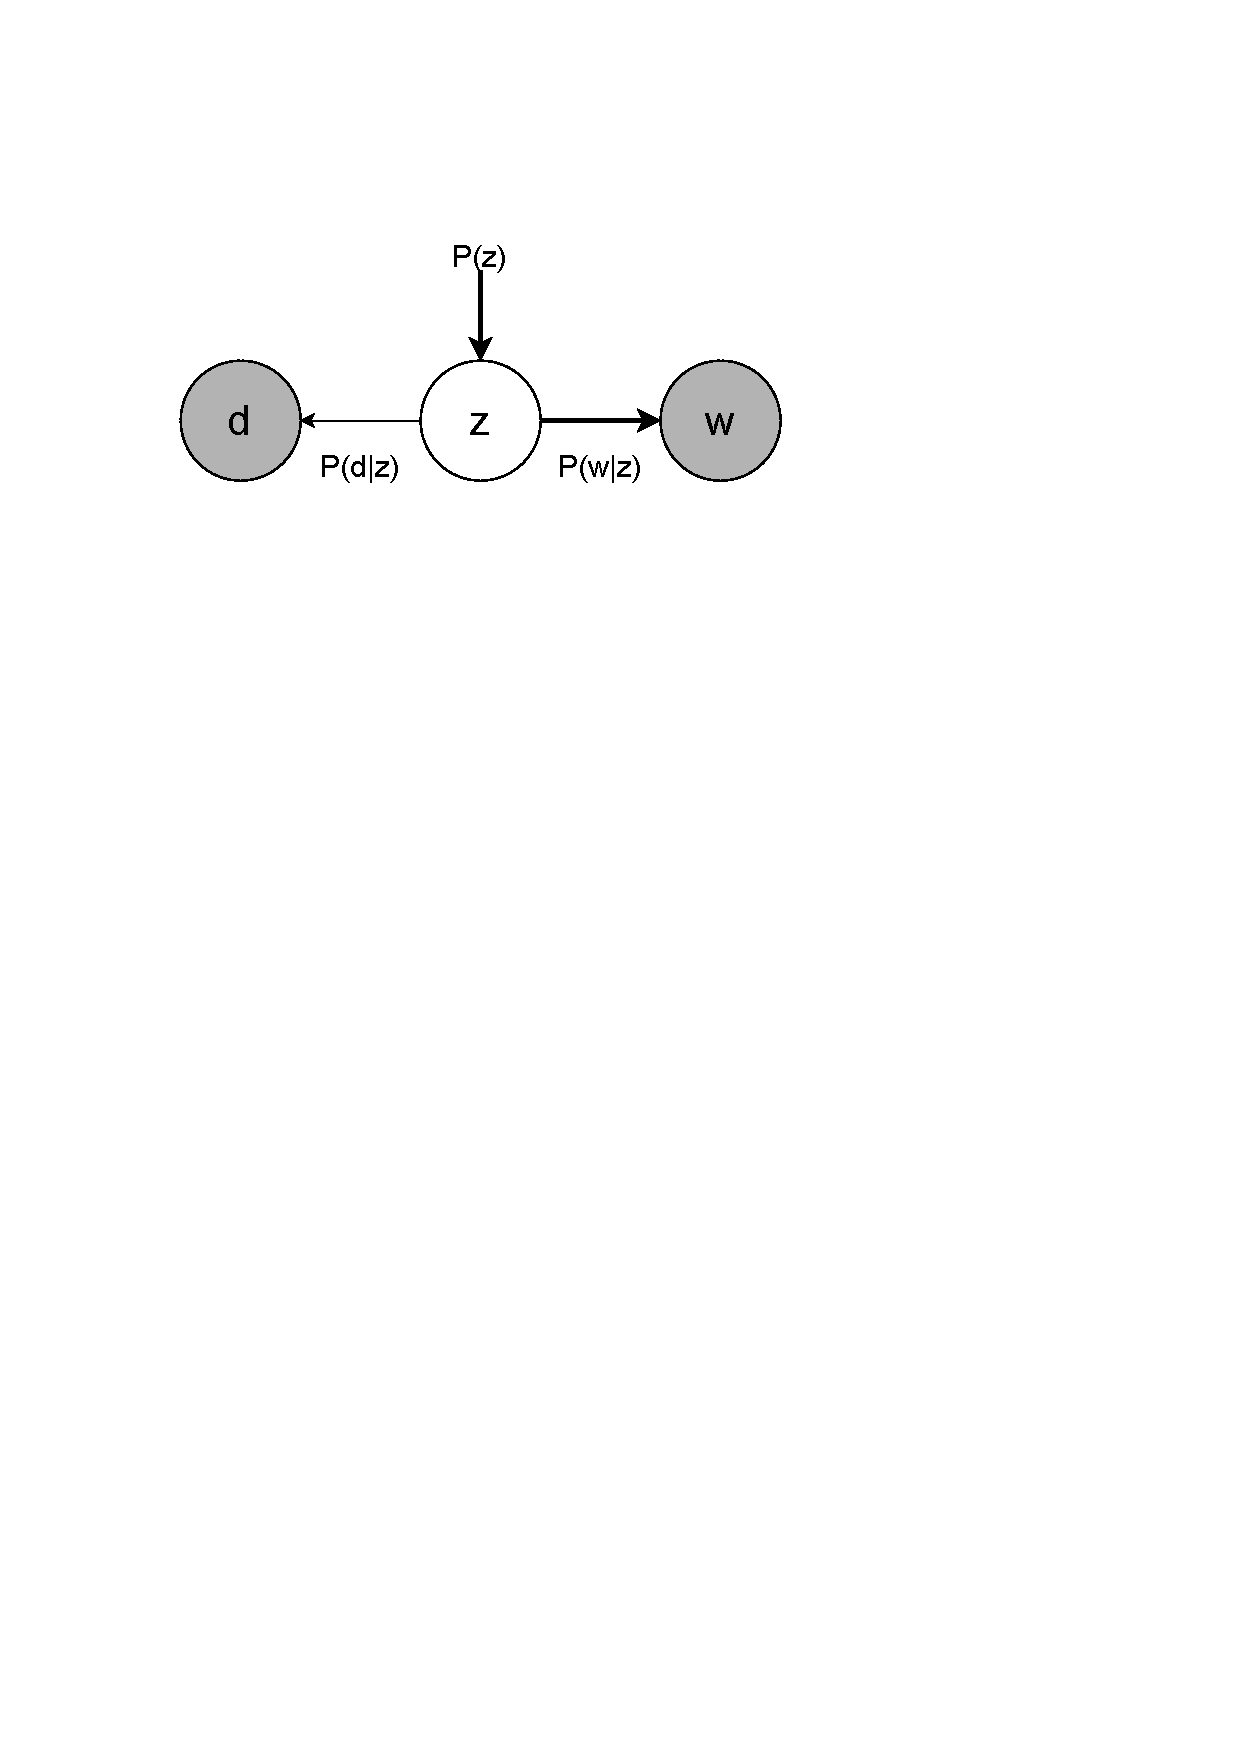
\includegraphics[width=8cm]{PLSA_graphical.pdf}
    \vspace{-7mm}
    \caption{PLSAグラフィカルモデル}
    \label{fig:mms}
    \vspace{5mm}
\end{figure}
文書dと単語wの同時出現頻度をN(d,w)とすると,対数尤度関数logLは式(3)として示せる.

\begin{equation}
\begin{split}
\rm{\log L= \sum_d\sum_wN(d,w)\log(P(d,w))}
\end{split}
\end{equation}
この対数尤度関数logLを最大にする確率変数P(z),P(d\verb+|+z),P(w\verb+|+z)をEMアルゴリズムによって推定する.なお推定する確率変数をモデルパラメータと呼ぶ.EMアルゴリズムとは混合分布モデルのパラメータ推定に利用できる学習アルゴリズムである.
zの確率分布P(z\verb+|+d,w)を予測するE(expectation)ステップと対数尤度関数の最大化をするM(maximization)ステップに計算ステップが分かれている.それぞれのステップで行われる計算の説明を順番に述べる.
式(4)はEステップの式である.初期値であるP(z),P(d\verb+|+z),P(w\verb+|+z)は絶対値が1以下のランダムな自然数に決定され,zの確率分布P(z\verb+|+d,w)を予測する.

\begin{equation}
\rm{P(z|d,w)=\frac{P(d|z)P(w|z)P(z)}{\sum_zP(d|z)P(w|z)P(z)}}
\end{equation}
式(5)(6)(7)はMステップの式であり,それぞれの式でモデルパラメータを求めている.

\begin{equation}
\rm{P(d|z)=\frac{\sum_wN(d,w)P(z|d,w)}{\sum_d\sum_wN(d,w)P(z|d,w)}}
\end{equation}

\begin{equation}
\rm{P(w|z)=\frac{\sum_dN(d,w)P(z|d,w)}{\sum_d\sum_wN(d,w)P(z|d,w)}}
\end{equation}

\begin{equation}
\rm{P(z)=\frac{\sum_d\sum_wN(d,w)P(z|d,w)}{\sum_d\sum_w\sum_zN(d,w)P(z|d,w)}}
\end{equation}
求めたモデルパラメータを式(2)に当てはめて式(3)の対数尤度関数の値を求める.対数尤度関数の値を最大化するまでEステップとMステップを交互に繰り返し,最適なモデルパラメータを求める.

\subsection{歌詞の印象推定手法}
この節では歌詞の印象推定手法について紹介する.

\subsubsection{印象の定義}
本稿で推定する印象とはRussellのAV平面上で表現する.AV平面は縦軸にArousalを,横軸にValenceを取る2次元平面である.Arousal軸は正の方向に興奮を,負の方向に弛緩を表す.そして,Valence軸は正の方向に快を,負の方向に不快を表す.
AV平面の4象限は大まかに喜怒哀楽の印象を表す.第1象限は喜びや幸福,興奮,驚きといった喜の感情グループを表す.第2印象は怒りや恐れ,嫌悪といった怒の感情グループを表す.第3章限は退屈や悲しみ,
憂鬱といった哀の感情グループを表す.第4象限は満足や穏やか,くつろぎといった楽の感情グループを表す.AV平面に歌詞データをプロットし,データが存在する象限から4つのグループの印象を推定できる.

\subsubsection{歌詞データの収集}
歌詞データの収集はUta-Net\footnote{https://www.uta-net.com/}から人気のアーティストの曲を6813曲収集した.本研究では6813曲から3000曲を無作為に選んだ.

\subsubsection{歌詞データの整形}
収集した歌詞データの中に一部英語が入っていたので,英語の歌詞を削除した.そして歌詞データを歌詞のフレーズごとに分解した.形態素解析器MeCabを用いて各フレーズから名詞・形容詞・動詞を抜き出した.歌詞から抜き出した単語の総数は109450語である.

\subsubsection{歌詞印象推定}
確率的潜在意味解析(PLSA)を利用する.歌詞のフレーズを文書dとし,フレーズ中に出現する単語を単語wと定義してモデルパラメータを推定した.
P(w\verb+|+z)はトピックから単語が観測される確率であるため,この確率の高い単語がトピックを表現する.
歌詞の印象を推定するためには潜在的なトピックzを印象に制限する必要がある.通常のPLSAは文書と単語の共起確率に着目して,潜在的なトピックを推定する手法である.よって必ず潜在的なトピックが印象を表現するとは限らない.
そのため,本間らの日本語版ANEWの単語データセットを事前知識として使用し,モデルパラメータをMAP推定することで潜在的なトピックにAV平面の各象限を表現する.
具体的に潜在的なトピックzを次の式(8)のようにAV平面の各印象として定義する.
\begin{equation}
\rm{z\in\{A+V+,A+V,-A-V,-A-V+\}}
\end{equation}
モデルパラメータの事前分布を共役事前分布を用いて式(9)に定義する.
\begin{equation}
\rm{P(θ)\propto\sum_w\sum_z(\alpha_{w,z}-1)\log P(w|z)}
\end{equation}
尤度関数は式(10)で表す.
\begin{equation}
\rm{\log P(w|z,D)=\sum}
\end{equation}
>>>>>>> feature/Abstract
%
\end{document}